\begin{figure}[!tb]
\begin{center}
\begin{tikzpicture}[]
\fill (0,0) node[inner sep=1pt] (A) {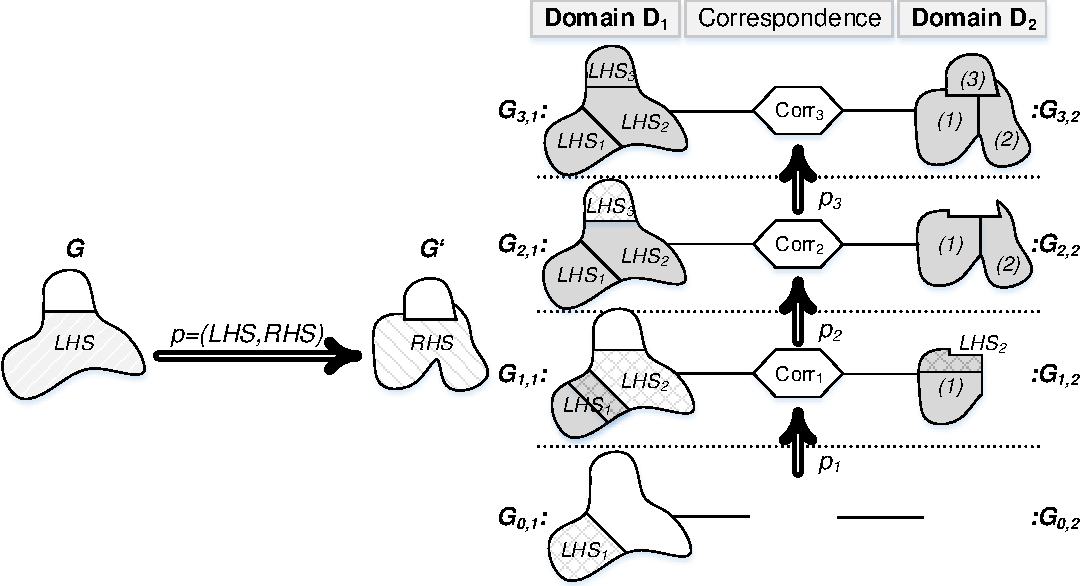
\includegraphics[width=\textwidth]{img/gen_intro/gts.pdf}};
\fill (3.55,-3.1) node[inner sep=1pt] (B) {\huge{$\varnothing$}};
\fill (5.9,-3.1) node[inner sep=1pt] (C) {\huge{$\varnothing$}};
\end{tikzpicture}
\end{center}
\caption{Rule-Based Graph Transformation Step (left) \& Model Transformation Sequence (right)}
\label{fig:sec-gen-intro-gratrafos:trafos}
\end{figure}

In this thesis, the theory of graph transformations is used as the consistent formal framework for defining models, model updates and model transformations as well as for performing model transformations and synchronisations \cite{Ehrig:2006:FAG:1121741,FAGT2}.
Therefore, models are represented by graphs.
We assume that most types of visual models as given in \cref{sec-gen-intro-models} can be represented by graphs.
Essentially, a graph consists of a set of nodes and a set of edges between nodes.
A model update defines which part of a graph is deleted and which part is added by the update.
A model transformation is defined in terms of a set of graph transformation rules.
A transformation rule (or production) $p=(\LHS,\RHS)$ contains a left-hand side (LHS) and a right-hand side (RHS).
When applying a rule $p$ to a graph $G$, then $G$ is transformed in the sense that LHS is replaced by RHS in $G$ leading to a new graph $G'$, denoted by $G \Trans{p} G'$ (cf. \cref{fig:sec-gen-intro-gratrafos:trafos} (left)).
Therefore, if $\LHS$ is a subgraph of $\RHS$ (i.e., $p$ only creates elements and therefore is non-deleting) then $\RHS \setminus \LHS$ is mainly added to $G$ while $\LHS$ is preserved by the rule application.
Otherwise, if intersection $\LHS \cap \RHS \neq \LHS$, then $\LHS \setminus \RHS$ is deleted in $G$, $\LHS \cap \RHS$ is preserved and $\RHS \setminus \LHS$ is added to $G$.
Note that this is an intuitive approach to graph transformations via set-theoretic operations $\setminus$ and $\cap$ on nodes and edges of graphs while technically, transformations are defined based on the category-theoretic concept of pushouts (cf. \cref{sec-gt-trafo}).

Commonly, model transformations from models in source domain $D_1$ (e.g., UML class diagrams) into models in target domain $D_2$ (e.g., entity-relationship diagrams) are defined based on a set of non-deleting graph transformation rules and performed by graph transformations, i.e., by applying transformation rules successively (so called model transformation sequences) as illustrated in \cref{fig:sec-gen-intro-gratrafos:trafos} (right).
The source (input) model (graph) $G_{0,1}$ of a transformation sequence in source domain $D_1$ is traversed step-wise in $n$ steps and target (output) model (graph) $G_{n,2}$ in target domain $D_2$ is constructed in parallel as follows:
\begin{enumerate}
\item At each step $i$ ($i \in \{1\ldots n\}$), a rule $p_i=(\LHS_i,\RHS_i)$ is applied to graph $(G_{i-1,1} \gets Corr_{i-1} \to G_{i-1,2})$ leading to a new graph $(G_{i,1} \gets Corr_{i} \to G_{i,2})$ where $G_{i,1}$ represents the graph part in domain $D_1$, $G_{i,2}$ the graph part in domain $D_2$ and $Corr_i$ is the correspondence that relates elements from $G_{i,1}$ with elements from $G_{i,2}$. - The model transformation sequence in \cref{fig:sec-gen-intro-gratrafos:trafos} (right) consists of three steps ($n=3$).
\item At the first step, only source graph $G_{0,1}$ is given as input to the transformation while $Corr_0$ and $G_{0,2}$ are empty (- nothing is transformed yet).
Therefore, by applying rule $p_1$, $\LHS_1$ in $G_{0,1}$ is marked as transformed in $G_{1,1}$ (by dark grey colouring) and $Corr_1$ with dark grey area $(1)$ are added (i.e., $\LHS_1$ in $G_{0,1}$ is transformed into $G_{1,2}=(1)$).
\item Analogously, in the following steps $i$, $\LHS_i$ in $(G_{i-1,1} \gets Corr_{i-1} \to G_{i-1,2})$ is transformed into $(i)$ in $G_{i,2}$.
Note that $\LHS_i$ may overlap with already transformed elements.
For example in Step 2 in \cref{fig:sec-gen-intro-gratrafos:trafos} (right), $\LHS_2$ overlaps with $\LHS_1$ in domain $D_1$ and with $(1)$ in domain $D_2$ and the result of Step 2 is that $\LHS_1 + \LHS_2$ in $D_1$ together are transformed into $(1)+(2)$ in $D_2$.
Step 3 in \cref{fig:sec-gen-intro-gratrafos:trafos} (right) shows the case where $\LHS_i$ in $D_1$ is transformed one-to-one without changing its structure into $(i)$ in $D_2$.
This is especially true for model refactorings where domains $D_1=D_2$, most steps are identical transformations and only a small part of the input graph is changed and therefore transformed into different structures.
\item The transformation sequence terminates and is complete, if the input graph $G_{0,1}$ is completely transformed, i.e., if $G_{0,1}$ is completely coloured (or marked) with dark grey such as is the case after Step 3 in \cref{fig:sec-gen-intro-gratrafos:trafos} (right).
\end{enumerate}
Thus, the rules for the model transformation are non-deleting, since, the source model is not transformed in-place but is only traversed step-wise and is rather preserved by the transformation while the target model is constructed in parallel.

Model synchronisations are performed based on model transformations w.r.t. a given model update.

In the literature, a variety of different graph transformation approaches is discussed with each having its own replacement mechanism for $\LHS$ by $\RHS$ in rule applications \cite{Rozenberg:1997:HGG:278918,Ehrig:1999:HGG:328523,graphgrammarhandbook99}. 
In this thesis, we use the algebraic approach to graph transformations \cite{Ehrig:2006:FAG:1121741} which was extended to model transformations and synchronisations in \cite{FAGT2}.
In \cref{sec-gen-intro-gt}, we review basic notions of algebraic graph transformation.
In \cref{sec-gen-intro-mt-ms-tgg}, we review basic technical notions and concepts of model transformations and synchronisations based on graph transformations.